\chapter{Linux als Kernel und Distro}
\label{cha:Linux}

\section{Was ist Linux?}

Unter dem Begriff Linux versteht man allgemein einen Überbegriff für freie Betriebssysteme, welche auf dem Linux Kernel basieren.\cite{LinuxWiki}
Der Linux Kernel wurde erstmals im Frühjahr 1992 unter der GNU GPL Lizenz für Intels x86 Architektur veröffentlicht.

Ein konkretes Linux Betriebssystem bezeichnet man als \textit{Linux Distribution} oder kurz Linux \textit{Distro}.
Eine Distribution besteht aus einem Linux Kernel, GNU Tools und Libraries, zusätzlicher Distro-spezifischer Software und manchmal auch einem Window System, einem Window Manager und einem Desktop Environment. Beispiele für solche Linux Distributionen sind Debian, Ubuntu, Arch Linux, openSUSE, Fedora und Linux on z.\cite{LinuxDistroWiki}

\section{Linux Kernel Architekturen}

Der Linux Kernel ist von monolithischer aber auch modularer Natur. Dies bedeutet, dass Funktionalität, welche der Kernel zwingend braucht, direkt eingebaut sind -- Funktionalitäten, welche aber nur bei ganz bestimmten Hardwarekomponenten gebraucht werden, können über sogenannte Kernel Module nachinstalliert und nachgeladen werden.
Der Linux Kernel übernimmt Aufgaben wie beispielsweise die Speicher- und Prozessverwaltung, Interprozesskommunikation, Geräte Verwaltung und Dateisysteme.
Nachfolgende Grafik zeigt eine Übersicht wichtiger Aufgaben des Linux Kernels im Zusammenspiel mit Hardware und den Userspace Anwendungen der Distribution:

\begin{figure}[h!]
\centering
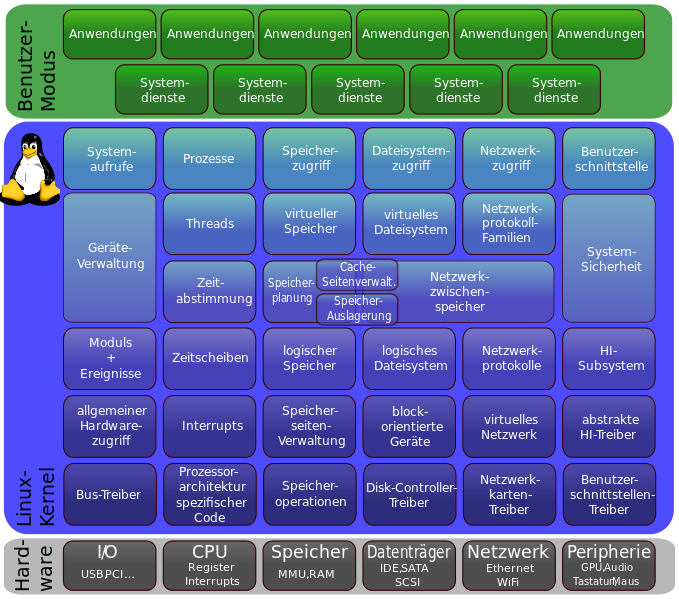
\includegraphics[width=.80\textwidth]{einleitung-kernel-struktur}
\caption{Linux Kernel Struktur\cite{KernelStruktur}.}
\label{fig:KernelStruktur}
\end{figure}

\newpage

Dieser modular-monolithischer Ansatz des Linux Kernels trägt nicht zuletzt zu seiner grossen Verbreitung auf unterschiedlichsten Architekturen und Plattformen bei.

Wikipedia führt eine Liste der Computer Architekturen, welche Linux unterstützt.\footnote{Siehe \url{https://en.wikipedia.org/wiki/List_of_Linux-supported_computer_architectures}}
Inzwischen sind dort über 100 Architekturen zu finden. Diese breite Abdeckung von Architekturen macht es möglich, dass Linux in beinahe alle Bereiche von Betriebssystem Umgebungen Einzug gefunden hat. Diese reicht von exotischen Umgebungen, wie Navigations- und Haushaltsgeräten, Digitalkameras, über Desktop- und Laptop Computern und Mobiltelefonen mit Android, bis hin zu Supercomputern und High Performance Computing Clusters mit Rocks Cluster Distribution.

So hat Linux auch seine Daseinsberechtigung auf dem Mainframe gefunden mit Linux on z, welches auf IBMs z Systems und IBMs LinuxONE läuft.

\section{Linux unter x86}
\label{sec:LinuxOnx86}

Die x86 Architektur war die erste unterstütze Architektur im Linux Kernel.
Dies aus dem einfachen Grund, weil Linus Torvalds, Autor und Maintainer von Linux, den Linux Kernel für seinen persönlichen Rechner entwickelt hat,
welcher eine Intel x86 CPU hatte.

\subsection{x86 Architektur im Rechenzentrum}

Seit Jahrzehnten halten sich x86 CPUs wacker im Kampf um die Marktanteile auf dem Server Markt.
Obwohl mit ARM eine eigentlich gute und vor allem effiziente Alternative existiert, machen die x86 Server immer noch einen Anzeil ueber 90\% aus.\cite{ARMServer}\cite{CommonWhyx86}

Linus Torvalds führt dies nicht auf die Architektur selbst zurück, sondern viel mehr auf das Ecosystem, welches sich um eine Architektur bildet:

\begin{quote}
"What matters is all the infrastructure around the instruction set, and x86 has all that infrastructure.
Being compatible just wasn’t as big of a deal for the ARM ecosystem as it has been traditionally for the x86 ecosystem."\cite{TorvalsQuote}
\end{quote}

Auch IBM versucht mit \textit{POWER8} und den aktuellen \textit{POWER9} Architekturen mehr Marktanteil im Serverbereich zu gewinnen.\cite{CommonWhyx86}
Neben IBMs eigenen Betriebssystemen unterstützt auch Linux\footnote{Seit Linux Kernel 4.6. Siehe \url{https://www.phoronix.com/scan.php?page=news_item&px=Linux-4.6-POWER9-POWER}} die POWER9 Architektur.
